\section{Frame Assembly}
The full frame and chassis of the vehicle were provided, however some modifications were necessary in order to incorporate the new design which allowed the 30:1 reduction box output shaft be coupled to the drive shaft of the drive box using a flexible coupling. In addition to the horizontal cross member, four vertical members were placed on the corners of the horizontal crossers to direct forces up through the rest of the frame, thus reducing the reliance on the welds to hold the weight of the vehicle. Furthermore, aluminum inserts were welded to the frame hole cutouts, in which brass bushings were pressed. The aluminum insert had a tapped hole with a grease nipple and a shoulder to separate both brass bushings, allowing grease to be put between the pivot and bushings. The frame assembly can be seen in Figure \ref{fig:battery_rack_and_frame_mount_drw}, and highlights both the horizontal and vertical supports. 

In order to accomodate the design allowing for the 30:1 worm gear reduction box output shaft to be coupled to the drive shaft of the drive box, the output hole in the frame needed to be raised by 10\,cm. The existing frame base member was 2x2x1/8'' rectangular tubing, however to increase the output hole height it was required that 2x8x3/16'' rectangular tubing was used. 

\begin{figure}[h]
\centering
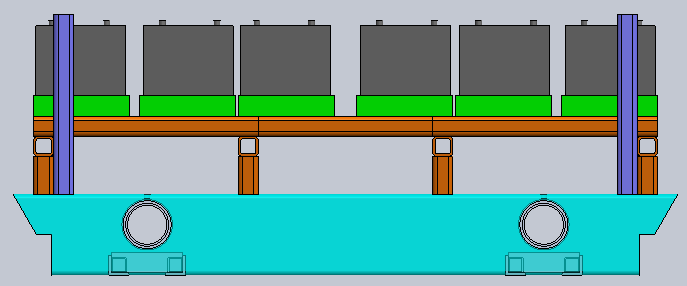
\includegraphics[width=0.7\linewidth]{./images/battery_rack_and_frame_mount_drw}
\caption{Frame Assembly Including Battery Rack and Frame Extension}
\label{fig:battery_rack_and_frame_mount_drw}
\end{figure}
 
\subsection{Design Constraints}
The design of the frame insert was constrained by the length of the vehicle, and needed to be made out rectangular tubing high enough to accomodate the output hole for the pivot. Since the frame shell could not be removed, the frame insert needed to be custom made to fit into the space where the old horizontal members were cut out. Many attempts were made at modelling the modifications, however the greatest success came from creating a cardboard template from which the desired geometry was finally cut out of the tubing. The vertical supports would need to rest on top of the rectangular tubing and extend into the top portion of the frame. The entire addition needed to be made out of the same grade of aluminum as the frame was to be weldable. 
\subsection{Functional Requirements}

\subsection{Analysis and Design}
\subsubsection{Frame}
\subsubsection{Aluminum Insert}
\subsubsection{Bushings}